\documentclass{beamer}
\usepackage[utf8]{inputenc}
\usepackage{listings}
\usepackage{xcolor}
\usepackage{tikz} % Added for diagrams
\usepackage{pgfplots} % Added for qualitative charts
\pgfplotsset{compat=1.18}
\usetikzlibrary{arrows,shapes,positioning,shadows,trees,mindmap,calc}

% Define custom colors for charts
\definecolor{chartblue}{RGB}{51, 102, 204}
\definecolor{chartred}{RGB}{220, 57, 18}
\definecolor{chartgreen}{RGB}{16, 150, 24}

% Theme selection
\usetheme{Madrid}
\usecolortheme{default}

% Title info (Will be replaced by Python)
\title{Assignment Solution}
\author{Solver\#42 AI Assistant}
\date{\today}

\begin{document}

\frame{\titlepage}

% Content (Will be replaced by Python)
\frame{
    \frametitle{Introduction to the IS-LM Model}
    \begin{itemize}
        \item The \textbf{IS-LM model} is a fundamental macroeconomic tool used to analyze the short-run fluctuations in an economy.
        \item It depicts the interaction between two markets:
        \begin{enumerate}
            \item \textbf{Goods Market (IS Curve):} Investment and Saving.
            \item \textbf{Money Market (LM Curve):} Liquidity preference and Money supply.
        \end{enumerate}
        \item The intersection determines the general equilibrium for interest rates ($r$) and real output/income ($Y$).
    \end{itemize}
}

\frame{
    \frametitle{The IS Curve (Goods Market Equilibrium)}
    \begin{itemize}
        \item \textbf{Definition:} Represents all combinations of interest rates ($r$) and output ($Y$) where the goods market is in equilibrium.
        \item \textbf{Equation:} $Y = C(Y-T) + I(r) + G$
        \item \textbf{Logic:}
        \begin{itemize}
            \item As the interest rate rises ($r \uparrow$), the cost of borrowing increases.
            \item Investment demand falls ($I \downarrow$).
            \item Lower investment reduces aggregate demand and output ($Y \downarrow$).
        \end{itemize}
        \item \textbf{Slope:} Downward sloping.
    \end{itemize}
}

\frame{
    \frametitle{The LM Curve (Money Market Equilibrium)}
    \begin{itemize}
        \item \textbf{Definition:} Represents all combinations of $r$ and $Y$ where the demand for real money balances equals the supply.
        \item \textbf{Equation:} $\frac{M}{P} = L(r, Y)$
        \item \textbf{Logic:}
        \begin{itemize}
            \item As income rises ($Y \uparrow$), the demand for money for transactions increases.
            \item With a fixed money supply ($M$), the interest rate must rise to restore equilibrium ($r \uparrow$).
        \end{itemize}
        \item \textbf{Slope:} Upward sloping.
    \end{itemize}
}

\frame{
    \frametitle{General Equilibrium Visualization}
    \begin{center}
    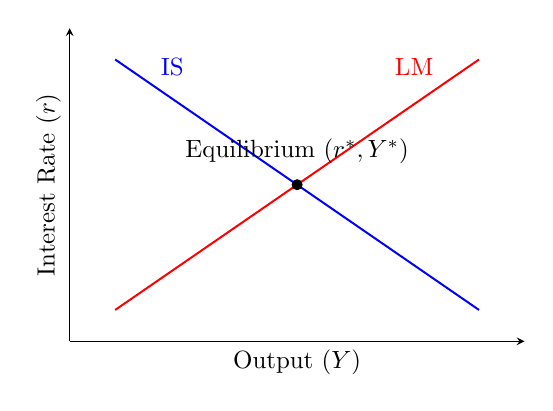
\begin{tikzpicture}[scale=0.9]
    \begin{axis}[
        axis lines = left,
        xlabel = {Output ($Y$)},
        ylabel = {Interest Rate ($r$)},
        ticks = none,
        xmin=0, xmax=5,
        ymin=0, ymax=5,
        width=8cm, height=6cm
    ]
    % IS Curve: Downward sloping (blue)
    \addplot [domain=0.5:4.5, samples=10, color=blue, thick] {5-x} node[pos=0.1, anchor=south west] {IS}; 
    
    % LM Curve: Upward sloping (red)
    \addplot [domain=0.5:4.5, samples=10, color=red, thick] {x} node[pos=0.9, anchor=south east] {LM};
    
    % Equilibrium Point
    \addplot[mark=*] coordinates {(2.5,2.5)};
    \node at (axis cs:2.5, 2.7) [anchor=south] {Equilibrium ($r^*, Y^*$)};
    
    \end{axis}
    \end{tikzpicture}
    \end{center}
    \vspace{-0.5cm}
    \begin{center}
    The point where IS intersects LM represents simultaneous equilibrium in both markets.
    \end{center}
}

\frame{
    \frametitle{Fiscal Policy Analysis}
    \begin{itemize}
        \item \textbf{Expansionary Fiscal Policy:} Increase in Govt. Spending ($G$) or Decrease in Taxes ($T$).
        \item \textbf{Effect:}
        \begin{itemize}
            \item Shifts the \textbf{IS Curve} to the \textbf{Right}.
        \end{itemize}
        \item \textbf{Result:}
        \begin{itemize}
            \item Output increases ($Y \uparrow$).
            \item Interest rates rise ($r \uparrow$).
        \end{itemize}
        \item \textit{Note:} The rise in $r$ can cause "Crowding Out" of private investment.
    \end{itemize}
}

\frame{
    \frametitle{Monetary Policy Analysis}
    \begin{itemize}
        \item \textbf{Expansionary Monetary Policy:} Central Bank increases Money Supply ($M$).
        \item \textbf{Effect:}
        \begin{itemize}
            \item Shifts the \textbf{LM Curve} to the \textbf{Right} (or Down).
        \end{itemize}
        \item \textbf{Result:}
        \begin{itemize}
            \item Interest rates fall ($r \downarrow$).
            \item Lower rates stimulate investment, increasing output ($Y \uparrow$).
        \end{itemize}
    \end{itemize}
}

\frame{
    \frametitle{Summary of Shocks}
    \begin{center}
    \renewcommand{\arraystretch}{1.5}
    \begin{tabular}{|c|c|c|c|}
    \hline
    \textbf{Policy Event} & \textbf{Curve Shift} & \textbf{Output ($Y$)} & \textbf{Interest ($r$)} \\
    \hline
    Govt Spending $\uparrow$ & IS shifts Right & Increases & Increases \\
    \hline
    Taxes $\uparrow$ & IS shifts Left & Decreases & Decreases \\
    \hline
    Money Supply $\uparrow$ & LM shifts Right & Increases & Decreases \\
    \hline
    Money Demand $\uparrow$ & LM shifts Left & Decreases & Increases \\
    \hline
    \end{tabular}
    \end{center}
}

\end{document}